\documentclass[a4paper]{article}
\usepackage{ fancyvrb, multicol}
\usepackage{ graphicx}

\usepackage[top=1.5 cm, bottom=2cm, left=1.5cm, right=1.5 cm]{geometry}
\begin{document}
\begin{center}
\vspace{3cm}
{\bf{\huge Chord book }}\\
\vspace{2cm}
USERNAME
\vspace{2cm}
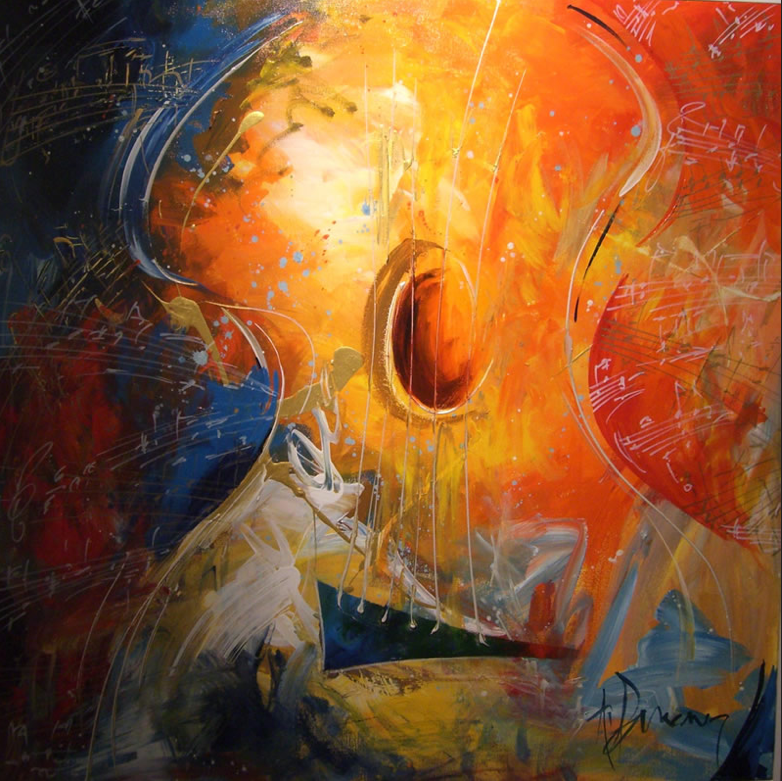
\includegraphics[scale=.6]{guitar2.png}\\
\vspace{1cm}
% \emph{A(nother) collection of all the songs I love to play}
\\
by Michele Esposito \\
\end{center}

\newpage
\tableofcontents
\newpage

## START ##
\section{Calle 13} % (fold)
\label{sec:Calle 13}
\subsection{Muerte en Hawaii} % (fold)
\label{sub:Muerte en Hawaii}

\begin{Verbatim}[commandchars=\\\{\}]

{\bf Intro: Eb}

{\bf Eb}
Yo he peliao con cocodrilos
{\bf                           Bb}
Me he balanceado sobre un hilo cargando más de 500 kilos
{\bf Cm }
Le he dao la vuelta al mundo en menos de un segundo
{\bf Ab                         Bb}
He cruzao 100 laberintos y nunca me confundo
{\bf Eb}
Respiro dentro y fuera del agua como las focas
{\bf G7}
Soy a prueba de fuego, agarro balas con la boca
{\bf Cm}
Mi creatividad vuela como los aviones
{\bf Ab                             Bb}
Puedo construir un cerebro sin leer las instrucciones


{\bf Ab                         Bb}
Hablo todos los idiomas de todos los abecedarios
{\bf Cm}
Tengo más vocabulario que cualquier diccionario
{\bf Ab                     Bb}
Tengo vista de águila, olfato de perro
{\bf Cm}
Puedo caminar descalzo sobre clavos de hierro
{\bf Ab}
Soy inmune a la muerte
{\bf Cm}
No necesito bendiciones porque siempre tengo buena suerte
{\bf Ab}
Ven conmigo a dar un paseo por el parque
{\bf              G7}
Porque tengo más cuentos que contarte que García Marqués


{\bf Eb}
Por ti, todo lo que hago lo hago por ti
{\bf                                   Cm}
Es que tú me sacas lo mejor de mí

Soy todo lo que soy
{\bf           Ab               Bb}
Porque tú eres todo lo que quiero (x2)


{\bf Eb}
Puedo brincar la cuerda con solo una pierna
{\bf     Bb}
Veo buen la oscuridad sin usar una linterna
{\bf Cm}
Cocino lo que quieras, yo soy todo un chef
{\bf       Ab          Bb}
Tengo sexo 24 - 7 todo el mes
{\bf Eb}
Puedo soplar las nubes grises pa que tengas un buen día
{\bf G7}
También se como comunicarme por telepatía
{\bf Cm}
Por ti, cruzo las fronteras sin visa
{\bf Ab                            Bb}
Y le saco una buena sonrisa a la Mona Lisa


{\bf Ab                       Bb}
Por ti, respiro antes de morirme
{\bf Cm}
Por ti voy a la Iglesia y escucho toda la misa sin dormirme
{\bf Ab                  Bb}
Sigo siendo el Rey, aunque no tenga reino
{\bf Cm}
Mi sudor huele a perfume y nunca me despeino
{\bf Ab                        Bb}
Se pelear todas las artes marciales
{\bf Cm}
También se como comunicarme con los animales
{\bf Ab}
Mientras más pasa el tiempo me veo más joven
{\bf                   G7}
Y esta canción la compuse sin escuchar como Beethoven

{\bf Eb}
Por ti, todo lo que hago lo hago por ti
{\bf                                   Cm}
Es que tú me sacas lo mejor de mí

Soy todo lo que soy
{\bf           Ab               Bb}
Porque tú eres todo lo que quiero (x2)
\end{Verbatim}
% subsection Muerte en Hawaii (end)
\newpage
\subsection{La Vuelta al Mundo} % (fold)
\label{sub:La Vuelta al Mu}

\begin{Verbatim}[commandchars=\\\{\}]
{\bf Bb}
No me regalen mas libros
{\bf A7}
{\bf Por que no los leo }
{\bf Dm}
Lo que he aprendido es por que lo veo 
{\bf          Bb                  A7}
Mientras mas pasan los anos me contradigo cuando pienso 
{\bf Dm                     G}
El tiempo no me mueve yo me muevo con el tiempo 

Soy las ganas de vivir 
las ganas de cruzar 
las ganas de conocer lo que hay despues del mar 
yo espero que mi boca nunca se calle 
tambien espero que las turbinas de este avion nunca me fallen 
no tengo todo calculado ni mi vida resuelta 
solo tengo una sonrisa y espero una de vuelta
yo confio en el destino y en la marejada 
yo no creo en la iglesia pero creo en tu mirada 
tu eres el sol en mi cara cuando me levanta 
yo soy la vida que ya tengo tu eres la vida que me falta 
asi que agarra tu maleta el bulto los motetes 
el equipaje tu valija la mochila con todos tus juguetes y 

{\bf B....                   A7....            Dm....}
dame la mano y vamos a darle la vuelta al mundo darle la vuelta al mundo 
{\bf G....}
darle al vuelta al mundo 
{\bf B....                   A7....            Dm....}
dame la mano y vamos a darle la vuelta al mundo darle la vuelta al mundo 
{\bf G....}
darle al vuelta al mundo 

la renta el sueldo el trabajo en la oficina 
lo cambie por las estrellas y por huertos de harina 
me escape de la rutina para pilotear mi viaje 
por que el cubo en el que vivia se convirtio en paisaje 
yo era un objeto esperando a ser ceniza 
un dia decidi hacerle caso a la brisa 
a irme resbalando detras de tu camisa 
no me convencio nadie me convencio tu sonrisa 
y me fui tras de ti persiguiendo mi instinto 
si quieres cambio verdadero pues camina distinto 
voy a escaparme hasta la constelacion mas cercana la suerte es mi oxigeno tus ojos son mi ventana 
quiero correr por 7 lagos en un mismo dia 
sentir encima de mis muslos el clima de tus nalgas frias 
llegar al tope de la sierra abrazarme con las nubes 
sumergirme bajo el agua y ver como las burbujas suben y

dame la mano y vamos a darle la vuelta al mundo darle la vuelta al mundo darle al vuelta al mundo 
dame la mano y vamos a darle la vuelta al mundo darle la vuelta al mundo darle al vuelta al mundo
\end{Verbatim}
\newpage
% subsection La Vuelta al Mu (end)
% section Calle 13 (end)
\section{Eva Cassidy} % (fold)
\label{sec:Eva Cassidy}
\begin{Verbatim}[commandchars=\\\{\}]
{\bf Intro:   C  G Em Am D G}

{\bf G   G     Bm       Bm}
Somewhere over the rainbow
{\bf C   Cm     G    G7}
    Way up high
{\bf C       Cm   G           Em}
There's a    land that I heard of
{\bf Am        D    G   G}
Once in a lullaby


{\bf G   G     Bm       Bm}
Somewhere over the rainbow
{\bf C   Cm        G    G7}
    Skies are blue
{\bf C   Cm  G               Em      Am}
And the dreams that you dare to dream
{\bf        D       G    G}
Really do come true


{\bf G                   G}
Some day I'll wish upon a star
{\bf     C                 Cm             Em Em  Em}
And wake up where the clouds are far behind me
{\bf       G                  G}
Where troubles melt like lemondrops
{\bf  F#7           F#7}
Away above the chimney tops
{\bf        Bm    Bm     Am   D}
That's where you'll find me

{\bf G   G     Bm       Bm}
Somewhere over the rainbow
{\bf C   Cm        G    G7}
    Bluebirds fly
{\bf C     Cm  G        Em}
Birds fly over the rainbow
{\bf Am           D         G   G}
Why then, oh why can't I?

{\bf G                   G}
Some day I'll wish upon a star
{\bf     C                 Cm             Em Em  Em}
And wake up where the clouds are far behind me
{\bf       G                  G}
Where troubles melt like lemondrops
{\bf  F#7           F#7}
Away above the chimney tops
{\bf        Bm    Bm     Am   D}
That's where you'll find me

{\bf G   G     Bm       Bm}
Somewhere over the rainbow
{\bf C   Cm        G    G7}
    Bluebirds fly
{\bf C     Cm  G        Em}
Birds fly over the rainbow
{\bf Am           D         G   G}
Why then, oh why can't I?

{\bf   G             G7}
If happy little bluebirds fly
{\bf   C}
Beyond the rainbow
{\bf Am      D        G}
{\bf Why, oh why can't I?}
\end{Verbatim}
\newpage
% section Eva Cassidy (end)
\section{The Cat Empire} % (fold)
\label{sec:The Cat Empire}
\subsection{The Chariot} % (fold)
\label{sub:The Chario}
\begin{Verbatim}[commandchars=\\\{\}]
{\bf            Verse 1:}
{\bf Em                        G}
This is a song that came upon me one night 
{\bf           Am}
When the news it had been telling me 
{\bf        C                D}
About one more war and one more fight
{\bf       Em }
And 'aeh' I sighed but then
{\bf      G}
I thought about my friends
{\bf          Am}
Then I wrote this declaration
{\bf          C              D}
Just in case the world end
{\bf  }


{\bf            Verse 2:}
Our guns
{\bf Em             G}
 We shot them in the things we said
{\bf         Am}
Ah we didn't need no bullets 
{\bf          C            D}
Cos we rely on some words instead 
{\bf Em}
Kill someone in argument
{\bf G}
Outwit them with our brains 
{\bf           Am}
And we'd kill ourselves laughing
{\bf          C                D}
At the funny things we'd say 



{\bf            Verse 3:}
And bombs 
{\bf Em              G}
  We had them saved for special times
{\bf           Am}
When the crew would call a shakedown 
{\bf      C            D}
We break down a party landmine 
{\bf Em}
Women that so sexy 
{\bf         G}
They explode us with their looks 
{\bf          Am}
Ah we blowing up some speakers 
{\bf           C              D        }
Jumping round till the ground shook 



{\bf            Verse 4:}
And missiles
{\bf Em                   G}
   They were the roadtrips that we launched
{\bf        Am}
T-t-tripping across this island 
{\bf             C              D}
Starting missions at the break of dawn
{\bf  Em}
Yawn and smile say 
{\bf         G}
What direction shall we take? 
{\bf Am}
Somewhere where it warm and wet 
{\bf C                        D}
This be the route we'd always take and 



{\bf            Chorus:}
{\bf Am                      Em}
  Our weapons were our instruments 
{\bf G           D          C}
Made from timber and steel 
{\bf               Am}
We never yielded to conformity 
{\bf       Em}
But stood like kings 
{\bf         G}
In a chariot that's riding on a 
{\bf    D}
Record wheel 

{\bf             Verse 5:}
{\bf            Em}
And our airforce flying 
{\bf             G}
When the frisbee in the sky 
{\bf          Am}
Have a session while we're smoking
{\bf              C           D}
Now we're feeling extra high 
{\bf           Em }
And we'd sneak into a carpark
{\bf             G}
With the skaties on our back 
{\bf             Am}
And we're flying down the levels howling 
{\bf          C                D}
On the attack now on the attack



{\bf            Verse 6:}
And battles 
{\bf Em                   G}
  They happened in these dancehalls 
{\bf            Am}
See we'd rather fight with music
{\bf     C               D}
Choosing one the rhythm war
{\bf Em}
Battle at these shakedowns 
{\bf          G}
And we battle at these gigs 
{\bf         Am}
We do battle in our bedrooms 
{\bf             C                D}
Made some sweet love to the beat 



           Bridge:
{\bf            Em}
Then our allies grew 
{\bf      G}
Wherever we would roam 
{\bf         Am }
See whenever we're together 
{\bf         C             D}
Any stranger feel at home 
{\bf       Em}
In a way we are an army 
{\bf           G}
But this army not destruct 
{\bf       Am}
No instead we're doing simple things
{\bf        C             D}
Good loving find it run amuck 



{\bf            Verse 7:}
{\bf Em}
This be a declaration 
{\bf    G}
Written about my friends
{\bf         Am}
It's engraved into this song 
{\bf          C               D}
So they know I'm not forgetting them 
{\bf       Em}
See maybe if the world contained
{\bf  G}
More people like these 
{\bf           Am}
Then the news would not be telling me
{\bf        C                   D}
About all that warfare endlessly and

{\bf  Chorus:}
\end{Verbatim}
\newpage
% subsection The Chario (end)
\subsection{The Lost Song} % (fold)
\label{sub:The Lost Song}
\begin{Verbatim}[commandchars=\\\{\}]
{\bf Dm    Bb    F    Am7}
{\bf  }
the words go a little like this... 
{\bf  }
{\bf VERSE 1: }
{\bf     Dm                                        Bb }
Oh, I had nine lives but I lost all of them 
{\bf               F }
And I've been searching in the night  
{\bf                          Am7 (and so on)...       }
And I've been searching in the rain 
I tried to find them, but they disappeared 
They walked away, they dressed in black 
They left my side and all I say is 
That I wasted time when I looked for them 
For now I know that things gone past  
Are never to be found again 
No never, never again 
I had nine lives but lost all of them... 
{\bf  }
{\bf VERSE 2: }
I had a plan but never finished it 
And I've been searching for the thought 
And I've been searching in a haze  
I try all days, to remember it 
But now the blueprint in my mind has gone 
My mind forgot the colour of direction 
And my eyes they see the hands 
That could've built that could've constructed 
The empire in my mind 
The empire I'll never find 
I had a plan but that was where it ended....ended..... 
{\bf  }
Depending on what version you have, various sections get repeated...
I'm sure you can work it out.
\end{Verbatim}
\newpage
% subsection The Lost Song (end)
\subsection{The Wine Song} % (fold)
\label{sub:The Wine Song}
\begin{Verbatim}[commandchars=\\\{\}]
{\bf INTRO}
(3/4 time)
{\bf | Dm | F+/C# | F | G/B | Bb | }
{\bf Dm/A | A7 | Dm |}

{\bf Dm        F+/C#    F        G/B}
Songs and melodies change and change
{\bf Bb}
And sway
{\bf          Dm/A           E7/Ab      A7}
But they still stay the same
{\bf Dm                F+/C#         G/C       G/B}
The songs that we sung when the dark days come
{\bf         Bb            Dm/A         A7          Dm}
Are the songs that we sung when we chased them away
{\bf Dm        F+/C#   F    G/B}
If I ever found a pot of gold
{\bf         Bb        Dm/A        E7/Ab         A7}
I'd buy bottles untold of the nectar of the vines
{\bf Dm           F+/C#      F           G/B}
I'm going to die with a twinkle in my eye
{\bf          Bb              Dm/A          A7            }
{\bf     Dm}
'cause I sung songs spun stories loved laughed and drank wine

{\bf Gm       Dm    A7   Dm}
Tomorrow is another day
{\bf Gm           Dm     A7       Dm}
The cats are out to play, to play
{\bf      Gm        Dm        A7       Dm}
That old rusty spaceship wants to sail
{\bf Gm       Dm    A7  Dm}
Into the milky way again
     Dm       Abdim   A7     | /A /B 
{\bf /C# |}
On a river of red red wine

[For this section, its really just the four chords written, but I included the bass 
notes as at the start when it is slow, those are very pronounced. But its just the chords 
with that Jewish Hora feel by alternating between the 5ths]

Dm   Dm/A (repeat)
{\bf Run...}
(let's have some)
Gm  Gm/D (repeat)
{\bf Fun...}
{\bf (we'll)}
Dm   Dm/A (repeat)
Drink...
(a toast to the)
A7   A7/E  (repeat)
{\bf Sun...}

{\bf [Same chords as verse 1]}

In summer the bushfires rage and rage
And rage
On such beautiful days
And we fight them with water that runs through the cracks
Water we're desperately trying to save
So I'll just live on wine and water my vines
And sleep on the wind with the fires right behind
And sing on the beaches and dance through the night
Oh we'll cry 'pass the wine, pass the wine, pass the wine'

{\bf Gm       Dm    A7   Dm}
Tomorrow is another day
{\bf Gm           Dm     A7       Dm}
The cats are out to play, to play
{\bf      Gm        Dm        A7       Dm}
That old rusty spaceship wants to sail
{\bf Gm       Dm    A7  Dm}
Into the milky way again
     Dm       Abdim   A7     | /A /B 
{\bf /C# |}
On a river of red red wine

[Again, same chords as before]

{\bf Run...}
(let's have some)
{\bf Fun...}
{\bf (we'll)}
Drink...
(a toast to the)
{\bf Sun...}

[Instrumental solo. This part is the same chords as the "run run run" section. The 
tricky part is the melody line, which I wont include, but if anyone actually wants it just 
contact me]

{\bf F         C         A7  Dm}
Oh what a beautiful day today!
{\bf Gm        F      C    F}
Today's a day to celebrate
{\bf F         C       A7        Dm}
Grab your bucket, grab your spade
{\bf Gm            F       C         F}
We're heading down to Half Moon Bay
{\bf F       C        A7     Dm}
I saw a plane go into a cloud
{\bf Gm            F         C           F}
I'm drunk I'm happy I'm singing and loud
{\bf F                  C         A7  Gm   A7  Bb}
                            [where the leading melody is C# D E D]
Two o'clock in the arvo, but hey that's allowed...
{\bf Gm                F         | C     C/E | F }
{\bf           A7 Dm}
I'm having a good time and of that I am proud
\end{Verbatim}
\newpage
% subsection The Wine Song (end)
% section The Cat Empire (end)
\section{Dire Straits} % (fold)
\label{sec:Dire Straits}
\subsection{Wild West End} % (fold)
\label{sub:Wild West E}
\begin{Verbatim}[commandchars=\\\{\}]
{\bf D                D            Em               G}
 Steppin' out to Angellucci's, for my coffee beans
{\bf D                 D      Em           G}
 checking out the movies, and the magazines
{\bf D             D          Em                         G}
 waitress she watches me, crossing from the Barocco bar
{\bf D              D     Em       G}
 I'm getting a pickup, for my steel guitar
{\bf            D           D   Em           G}
 I saw you walking out,      Shaftsbury Avenue
{\bf D          D                Em      G}
 excuse me talking, I wanna   marry you
{\bf D        D                        Em                  G}
 this is seventh heaven street to me, don't you be so proud
{\bf D                    D      Em       G}
 You're just another angel,   in the crowd. 

{\bf              D              D         Em        G}
	And I'm walking in the wild west end
{\bf      D              D         Em        G}
	Walking in the wild west end
{\bf      D                 D         Em        G     D/A G/C /C D/}
	Walking with your wild best friend


And my conductress on the number nineteen, she was a honey
pink toenails and hands all dirty with the money
greasy greasy greasy hair, easy smile
made me feel nineteen, for awhile
and I went down to Chinatown
in the backroom it's a man's world, all the money go down
Duck inside the doorway, gotta duck to eat
right now feels all right now, you and me we can't beat walking -

{\bf Chorus}

And a gogo, dancing girl, yes I saw her
the deejay, he say, here's Mandy for ya
I fell all right to see her, but she's paid to do that stuff
She's dancing high, I move on by, the close ups can get rough
when you're walking in the wild west end . . .

{\bf Chorus / Tag}
\end{Verbatim}
\newpage
% subsection Wild West E (end)
% section Dire Straits (end)
\section{Grateful Dead} % (fold)
\label{sec:Grateful Dead}
\subsection{Friend Of The Devil} % (fold)
\label{sub:Friend Of The Devil}

\begin{Verbatim}[commandchars=\\\{\}]
{\bf Intro:}

{\bf / G - - - / - - - - / C - - - / - - - - / x4}

{\bf G (2)}
I lit out from Reno,
{\bf             C (2)}
I was trailed by twenty hounds
{\bf  G (2)}
Didn't get to sleep that night
{\bf                C (2)}
'Till the morning came around.

{\bf Chorus:}
{\bf   D (2)}
Set out runnin' but I take my time
{\bf      Am (2)}
A friend of the devil is a friend of mine
{\bf    D (2)}
If I get home before daylight,
{\bf    Am (2)                                 D (4)}
I just might get some sleep tonight.

Ran into the devil, babe,
He loaned me twenty billf
I spent the night in Utah
In a cave up in the hills.

{\bf Chorus}

I ran down to the levee
But the devil caught me there
He took my twenty-dollar bill
And vanished in the air.

{\bf Chorus}

{\bf Bridge:}
{\bf   D (2)}
Got two reasons why I cry
{\bf     D (2)}
Away each lonely night,
{\bf        C (2)}
The first one's named Sweet Anne Marie,
{\bf           C (2)                        }
And she's my hearts delight.
{\bf         D (2)}
The second one is prison, baby,
{\bf           D (2)}
{\bf The sheriff's on my trail,}
{\bf       Am (2)}
And if he catches up with me,
{\bf         C                    D (4)}
I'll spend my life in jail.

Got a wife in Chino, babe,
And one in Cherokee
The first one says she's got my child,
But it don't look like me.

{\bf Chorus}

{\bf Instrumental Verse & Chorus}

{\bf Repeat from Bridge, End at Chorus (hold last D)}
\end{Verbatim}
\newpage
% subsection Friend Of The Devil (end)
% section Grateful Death (end)
\section{Jimi Hendrix} % (fold)
\label{sec:Jimi Hendrix}
\subsection{All Along the Watchtower} % (fold)
\label{sub:All Along the Watchtower}
\begin{Verbatim}[commandchars=\\\{\}]
{\bf 	  Am                G                F           G }
There must be some kind of way out of here
Said the joker to the thief
There's too much confusion
I can't get no relief
Buisness men they drink my wine
Plowmen dig my earth
None would ever compromise
Nobody of this world

No reason to get excited
The thief he kindly spoke
There are many here among us
Who feel that life is but a joke
But you and I we've been through that
And this is not our place
So let us stop talking falsely now
The hour's getting late

All along the watchtower
Princess kept the view
While all the women came and went
Barefoot servants too
Outside in the cold distance
A wildcat did growl
Two riders were approaching
And the wind began to howl

All along the watchtower
All along the watchtower
All along the watchtower
\end{Verbatim}
\newpage
% subsection All Along the Watchtower (end)
\subsection{Hey Joe} % (fold)
\label{sub:Hey Joe}
\begin{Verbatim}[commandchars=\\\{\}]
{\bf 	  C       G  D      A                               }
  Hey Joe    where ya' goin' with that  
{\bf / E - - - / - - E7 - / E - - - / - - E7 - / }
gun in your hand? 
{\bf          C       G  D      A   }
I said, hey Joe      where ya goin' with that  
{\bf / E - - - / - - E7 - / E - - - / - - E7 - / }
gun in your hand?  
{\bf C                            G                      D    A                            }
   I'm goin' down to shoot my old lady.   I caught her messin' round with  
{\bf / E - - - / - - E7 - / E - - - / - - E7 - / }
another man  
{\bf C                           G                      D                    A   }
  I'm goin' down to shoot my old lady.  You know I caught her messin' round with  
{\bf / E - - - / - - E7 - / E - - - / - - E7 - / }
another man. 
{\bf C        G  D  A }
  Hey Joe,        I heard you shot your 
{\bf / E - - - / - - E7 - / E - - - / - - E7 - / }
woman down you shot her down down 
{\bf C        G  D  A }
   Hey Joe,     I heard you shot your  
{\bf / E - - - / - - E7 - / E - - - / - - E7 - / }
lady down, You shot her down to the ground 
{\bf C             G                D          A }
   Yes, I did, I shot her,  you know I caught her messin' 'round,  
{\bf / E - - - / - - E7 - / E - - - / - - E7 - / }
messin' 'round town 
{\bf C          G                   D                   A }
  Yes, I did, I shot her,  you know I caught my old lady messin'  
{\bf / E - - - / - - E7 - / E - - - / - - E7 - / }
'round the town, and I gave her the gun, I shot her 
Guitar solo (3 Progressions) 
{\bf C        G  D  A }
   Hey Joe,     where you gonna run to  
{\bf / E - - - / - - E7 - / E - - - / - - E7 - / }
now, where you gonna run to? 
{\bf C  G                   D  A }
   Hey Joe, I said,     where you gonna  
{\bf / E - - - / - - E7 - / E - - - / - - E7 - / }
run to now, Where you, where you gonna go? 
{\bf C                 G                    D  A }
   I'm goin' way down south,      way down  
{\bf / E - - - / - - E7 - / E - - - / - - E7 - / }
Mexico way, alright 
{\bf C                 G                    D  A }
   I'm goin' way down south,     way down where  
{\bf / E - - - / - - E7 - / E - - - / - - E7 - / }
I can be free--ain't no one gonna find me 
{\bf C               G                    D                         A }
   Ain't no hangman gonna,   He ain't gonna put a rope around  
{\bf / E - - - / - - E7 - / E - - - / - - E7 - / }
{\bf me,  }
Repeat Progression 
{\bf End on E }
\end{Verbatim}
\newpage
% subsection Hey Joe (end)
\subsection{The Wind Cries Mary} % (fold)
\label{sub:The Wind Cries Mary}
\begin{Verbatim}[commandchars=\\\{\}]
{\bf  |:  Eb    E  F     Eb   E  F :| }
{\bf  }
{\bf C             Bb                 F }
After all the jacks are in their boxes 
{\bf C                   Bb          F }
And the clowns have all gone to bed 
{\bf C                      Bb            F }
You can hear happiness staggering on down the street 
{\bf G         Bb         Eb E F }
Footsteps dressed in red 
{\bf G       Bb            Eb E F  Eb E F }
And the wind whispers Mary 
{\bf  }
{\bf  }
{\bf C          Bb       F }
A broom is drearily sweeping 
{\bf C                       Bb          F }
Up the broken peices of yesterday's life 
{\bf C           Bb       F }
Somewhere a queen is weeping 
{\bf G           Bb          Eb E F }
Somewhere a king has no wife 
{\bf G            Bb    Eb E F  Eb E F }
And the wind cries Mary 
{\bf  }
{\bf  }
{\bf SOLO  |: F  Eb  Bb  Ab :| 3x    G  Bb  Db  F }
{\bf  }
{\bf  }
{\bf C                       Bb     F }
The traffic lights turn blue tomorrow 
{\bf C                       Bb         F }
And shine the emptyness down on my bed 
{\bf C               Bb   F }
The tiny island sags downstream 
{\bf G                   Bb       Eb E F }
Cause the life that lived is dead 
{\bf G            Bb      Eb E F  Eb E F }
And the wind screams Mary 
{\bf  }
{\bf  }
{\bf C             Bb     F }
Will the wind ever remember 
{\bf C                Bb           F }
The names it has blown in the past 
{\bf C                        Bb           F }
With its crutch, its old age, and its wisdom 
{\bf G                         Bb     Eb E F }
It whispers no, this will be the last 
{\bf G            Bb    Eb E F  Eb E F  Eb E F  Eb E F }
And the wind cries Mary 
\end{Verbatim}
\newpage
% subsection The Wind Cries Mary (end)
% section Jimi Hendrix (end)
\end{document}
